\documentclass[10pt,a4paper]{article}
\usepackage[T1]{fontenc}
\usepackage[utf8]{inputenc}
\usepackage{lmodern}
\usepackage[margin=22mm]{geometry}
\usepackage{amsmath,amssymb,booktabs,graphicx,microtype}
\usepackage[numbers,sort&compress]{natbib}
\usepackage[font=small,labelfont=bf]{caption}
\usepackage{xcolor}
\usepackage[colorlinks=true,allcolors=blue!45!black]{hyperref}
\setlength{\parindent}{1em}
\setlength{\parskip}{2pt}
\setlength{\textfloatsep}{10pt}
\setlength{\intextsep}{10pt}
\setlength{\bibsep}{2pt}
\renewcommand{\topfraction}{0.92}
\renewcommand{\bottomfraction}{0.85}
\renewcommand{\textfraction}{0.08}
\renewcommand{\floatpagefraction}{0.85}
\renewcommand{\bibfont}{\footnotesize}
\newcommand{\ChecksPassed}{72}
\newcommand{\ChecksSkipped}{2}
\newcommand{\ChecksFailed}{0}

\title{\vspace{-15mm}Epiplexity and Transfer in\\Synthetic Time-Series Pretraining}
\author{\normalsize Danila Chernousov \quad Mark Ikonnikov \quad Daniil Kazachkov \quad Alexey Kravatskiy\\[2pt]
\small Moscow Institute of Physics and Technology}
\date{21 October 2026}
\hypersetup{
pdftitle={Epiplexity and Transfer in Synthetic Time-Series Pretraining},
pdfauthor={Danila Chernousov, Mark Ikonnikov, Daniil Kazachkov, Alexey Kravatskiy},
pdfsubject={Synthetic time-series pretraining and excess prequential loss},
pdfkeywords={epiplexity, time series, synthetic data, prequential coding, forecasting}
}

\begin{document}
\maketitle
\vspace{-7mm}
\begin{abstract}
Synthetic pretraining offers controllable forecasting tasks, but selecting useful
data distributions remains difficult. We investigate whether excess prequential
loss, a learning-curve proxy for epiplexity, predicts transfer to real time series.
Using \texttt{episynth}, we compare eleven synthetic priors at training budgets
of approximately 2 and 40 million windows. A probabilistic Moirai transformer is
trained from scratch on each prior and evaluated on 55 short-term GIFT-Eval
configurations. KernelSynth achieves the best aggregate transfer at both budgets,
with geometric mean CRPS ratios to seasonal naive of 0.678 and 0.639.
However, excess area has weak rank association with transfer across all eleven
priors ($\rho=-0.18$ and $0.00$). Stronger associations depend on exploratory
subset selection. Endpoint averaging and rare forecast failures substantially
affect the measured relationship. Our results identify useful synthetic priors
under a fixed forecasting protocol, while showing that excess area alone does
not establish a reliable rule for selecting pretraining data.
\end{abstract}

\section{Introduction}
Synthetic data make the pretraining distribution an experimental choice.
For forecasting, one can generate trends, periodic signals, stochastic innovations,
or chaotic trajectories in arbitrary quantities. These distributions differ in
both predictability and the structure a model can learn. A low synthetic
prediction loss therefore need not imply useful representations for real series.
The practical question is which property of a synthetic prior can guide data
selection before an expensive downstream evaluation.

Epiplexity describes structure accessible to a computationally bounded
observer~\cite{finzi2026}. This suggests a testable hypothesis: priors from which
a forecasting model acquires more structure should yield better transfer.
Following our initial study design~\cite{chernousovtalk,chernousovproposal},
we examine this hypothesis through excess prequential loss: the accumulated
online prediction loss above a held-out endpoint. We compare eleven priors at
two data budgets using one architecture and a common evaluation protocol.

Our contributions are threefold. We describe \texttt{episynth}, a reproducible
pipeline connecting synthetic tasks, probabilistic training, excess-loss
estimation, and forecasting evaluation. We analyze 22 primary runs and one
initialization repeat, totaling 501,992,448 training windows. Finally, we show
that aggregate transfer and excess area have weak full-set association, and
identify endpoint choice and forecast tails as material sources of sensitivity.

\section{Related work}
Finzi et al.~\cite{finzi2026} motivate prequential epiplexity estimates; Su et
al.~\cite{su2026} use epiplexity for language-model data selection and generation.
Its forecasting value requires validation: synthetic corpus composition and
architecture affect time-series transfer~\cite{nagpal2026}. Chronos introduces
KernelSynth data~\cite{ansari2024}; Moirai supplies our probabilistic
transformer~\cite{woo2024}, and GIFT-Eval the benchmark~\cite{aksu2024}.
Prior-fitted networks motivate approximate Bayesian prediction from synthetic
tasks~\cite{muller2022}; information-theoretic in-context learning analysis
informs the proposed oracle decomposition~\cite{jeon2024}.

\section{Methodology}
\subsection{Problem formulation}
Let $g$ denote a synthetic prior over context--target pairs $(C,Y)$, where
$Y=(Y_1,\ldots,Y_h)$. A probabilistic forecaster $q_\theta$ is trained with loss
$\ell_\theta(C,Y)=-\sum_{t=1}^{h}\log q_\theta(Y_t\mid C)$.
We ask whether the excess loss accumulated while learning $g$ predicts the
model's subsequent forecasting error on real datasets. Model size and training
windows are fixed within each comparison; the prior is the experimental variable.

\subsection{Synthetic task distributions}
The eleven priors cover Gaussian-process kernels (KernelSynth), exponential
smoothing (ETS), periodic waveforms, switching stochastic differential equations
(SDE), steps, composed trend, seasonality and irregularity (TSI), ARIMA, fractional
Brownian motion (fBm), GARCH volatility, chaotic dynamics, and TimeSynth signals.
A seeded generator produces a length-1024 series. A separate seeded procedure
selects a start, context $C$ of length $c$, and a future target $Y$ of horizon
$h=64$. The saved configurations sample 492 context lengths between 13 and 512,
with weights derived from GIFT-Eval history lengths. Short contexts are padded
and masked; future values are excluded from context normalization. Uniform
dequantization of width $10^{-3}\sqrt{\widehat{\mathrm{Var}}(C)+10^{-5}}$ smooths
the observations. The same series seed produces the same window independently
of batch composition or worker count.

\subsection{Probabilistic model and training}
The observer is a Moirai 1.x port trained from scratch: six transformer layers,
width 384, patch size 32, and 10,746,600 parameters. Its density head mixes
Student-$t$, fixed-scale Gaussian (scale $10^{-3}$), and log-normal components,
with context scaling. Table~\ref{tab:budgets} gives the completed budgets.

\begin{table}[htbp]
\centering\small
\caption{Training series. Counts are per prior; the extra seed belongs to series 2.}
\label{tab:budgets}
\begin{tabular}{@{}lrrl@{}}
\toprule
Series & Windows $N$ & Optimizer steps & Training data access\\
\midrule
1 (2M) & 1,999,872 & 1,953 & Precomputed corpora\\
2 (40M) & 39,999,488 & 39,062 & Online; KernelSynth precomputed\\
\bottomrule
\end{tabular}
\end{table}

Both series use batch size $B=1024$, AdamW with learning rate $10^{-3}$,
200 warmup steps, weight decay 0.1, $\beta=(0.9,0.98)$, $\epsilon=10^{-6}$,
and gradient clipping at 1. The EMA time constant is 2\% of the total step budget.
Training uses bfloat16. At 1, 2, 5, 10, 20, 50, and 100\% of the budget, raw and
EMA weights are scored on 100,000 held-out windows, starting at seed $10^9$.
Additional float32 scores are saved; the area below uses the matching bfloat16
floor. Primary runs share initialization seed 0 and training seeds starting at 0;
Waveform additionally uses initialization seed 1. The two budgets therefore
share seed ranges and are not independent replications. Windows and model size
are matched within a series; hardware and data-generation costs vary.

\subsection{Excess prequential loss as a structural proxy}
For time-bounded probabilistic programs $\mathcal P_T$, formal epiplexity is the
model-description part of an optimal two-part code~\cite{finzi2026}:
\begin{equation}
 P_T^\star\in\arg\min_{P\in\mathcal P_T}
 \{|P|+\mathbb E[-\log_2 P(Y\mid C)]\},\qquad S_T(Y\mid C)=|P_T^\star|.
\end{equation}
The programs must both sample and evaluate probabilities within the time bound.
The experiment estimates an algorithm-dependent learning-curve proxy. Let $u_k$
be the mean negative log density per target point in batch $k$, measured
\emph{before} its update, and $\widehat\ell_N^{\rm EMA}$ the final held-out EMA loss
in nats per window. The signed excess area is
\begin{equation}
 A_N=Bh\sum_{k=1}^{K}u_k-N\widehat\ell_N^{\rm EMA},
 \qquad \widehat S_N=A_N/\ln 2,\qquad N=BK.
 \label{eq:area}
\end{equation}
All reported areas use million nats; division by $\ln 2$ yields bits.
Figure~\ref{fig:training} shows the underlying curves. A common conditional-entropy
term cancels in the expected excess loss: for fresh independent tasks and an
unbiased endpoint estimate, it becomes a sum of differences between the online
and endpoint conditional KL divergences to the true prior predictive.
This motivates measuring learning progress, but does not identify the optimal
program in the formal definition.

\begin{figure}[htbp]
\centering
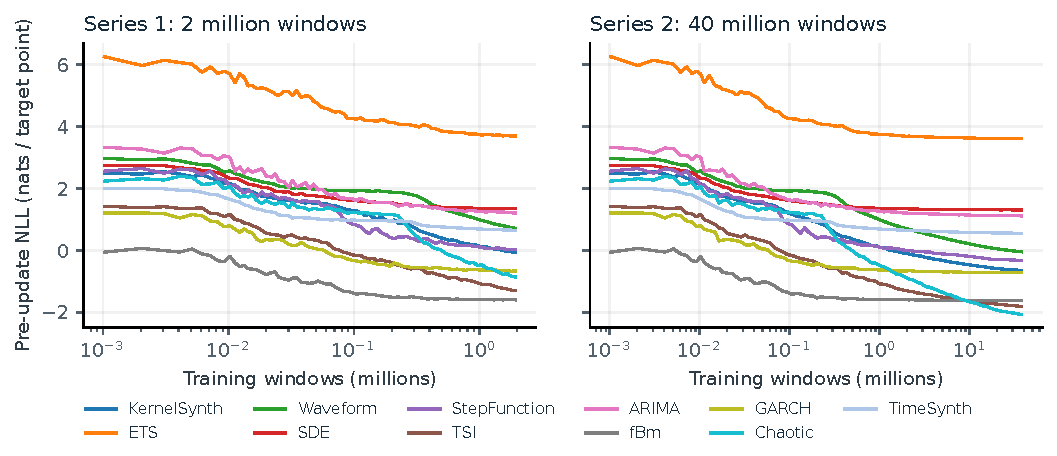
\includegraphics[width=\linewidth]{figures/training_results.pdf}
\caption{Saved pre-update training losses for the eleven primary runs. Curves
average log-spaced groups of steps for display; Eq.~\eqref{eq:area} uses every
exported step. Negative continuous-density losses are valid.}
\label{fig:training}
\end{figure}

The floor matters. Online losses use raw weights, whereas the primary endpoint
uses EMA weights. Relative to a raw endpoint, this adds
$N(\widehat\ell_N^{\rm raw}-\widehat\ell_N^{\rm EMA})$ to the area. A floor error
$\delta$ shifts $A_N$ by $-N\delta$; positive clipping would define another
statistic. Continuous-density losses also require consistent units and
quantization to admit a coding interpretation. We retain the repository's
original-unit densities and its signed area throughout.

\subsection{Transfer metrics and uncertainty}
The final EMA model is evaluated without fine-tuning on 55 short-term GIFT-Eval
configurations. For metric $m$, we normalize by the saved seasonal-naive baseline
and weight each configuration equally:
\begin{equation}
 R_g^{(m)}=\exp\left\{\frac1{55}\sum_{j=1}^{55}
 \log\frac{m_{g,j}}{m_{{\rm naive},j}}\right\}.
 \label{eq:quality}
\end{equation}
Smaller ratios are better; $R<1$ beats the baseline. The main metric is the
sample-based \texttt{scaled\_crps}; the separate nine-quantile
\texttt{mean\_weighted\_sum\_quantile\_loss} field is not substituted for it.
MASE, median ratios, and average configuration ranks are sensitivity checks.
We compute Spearman correlations across the eleven generator families and 95\%
percentile intervals from 10,000 paired bootstrap resamples of families (seed 0).
These intervals describe variation across the small set of priors, not training
seed uncertainty. The 55 configurations include related datasets/frequencies
and are not 55 independent training replications.

\section{Implementation}
The \texttt{episynth} package separates four algorithms: seeded task generation,
probabilistic training with AdamW and EMA, excess prequential-loss estimation,
and transfer evaluation with ranking uncertainty (Appendix~\ref{sec:algorithms}).
Generators and precomputed corpora share a batch interface; window draws depend
on series seeds, allowing parallel generation without changing task identity.
The trainer records pre-update losses and saves model, optimizer, and EMA states
for resumption. The analysis operates on these logs separately from training;
batch means suffice to reconstruct the signed area. Evaluation writes per-window
statistics and configuration summaries for the model and seasonal naive.
Source, configurations, and experiment outputs are available in the
\href{https://github.com/intsystems/Epiplexity}{project repository}.

\section{Experimental evaluation}
We use the completed training series of 19--20 October 2026~\cite{chernousovresults}.
All 23 runs are included; the additional Waveform initialization is reported
separately from the eleven-family comparisons. Statistics are recomputed from
the archived loss curves, held-out checkpoints, and forecast summaries.
\subsection{Training budget and downstream performance}
Table~\ref{tab:results} reports all primary runs and the additional initialization.
KernelSynth achieves the lowest aggregate CRPS ratio at both budgets and beats
seasonal naive in 50 of 55 configurations in each series. ETS ranks second.
Increasing the budget improves aggregate CRPS for eight of eleven primary priors;
Waveform, fBm, and Chaotic worsen. StepFunction improves substantially, from
1.607 to 0.839. Thus more optimization helps many priors, but does not uniformly
improve transfer.

\begin{table}[htbp]
\centering\small
\caption{Recomputed signed EMA-floor area $A$ (million nats) and geometric mean
metric ratios to seasonal naive. Lower metric ratios are better. Seed 0 unless
specified; the seed-1 repeat is excluded from the eleven-family correlations.}
\label{tab:results}
% Generated by analyze_runs.py; values come from run_statistics.csv.
\begin{tabular}{@{}lrrrrr@{}}
\toprule
 & \multicolumn{2}{c}{Series 1: 2M} & \multicolumn{3}{c}{Series 2: 40M}\\
\cmidrule(lr){2-3}\cmidrule(l){4-6}
Prior & $A$ & CRPS & $A$ & CRPS & MASE\\
\midrule
KernelSynth & 68.4 & \textbf{0.678} & 926.1 & \textbf{0.639} & 0.828 \\
ETS & 26.7 & 0.731 & 138.6 & 0.717 & 0.941 \\
Waveform & 70.9 & 0.818 & 1061.2 & 1.373 & 0.986 \\
SDE & 11.0 & 0.872 & 34.6 & 0.861 & 1.142 \\
StepFunction & 49.5 & 1.607 & 588.3 & 0.839 & 1.092 \\
TSI & 64.8 & 0.803 & 765.9 & 0.776 & 1.028 \\
ARIMA & 24.2 & 0.847 & 154.5 & 0.833 & 1.089 \\
fBm & 9.6 & 0.853 & 40.6 & 0.867 & 1.110 \\
GARCH & 16.6 & 0.879 & 100.9 & 0.874 & 1.116 \\
Chaotic & 126.2 & 1.171 & 1956.6 & 1.285 & 1.616 \\
TimeSynth & 15.3 & 0.974 & 114.9 & 0.851 & 1.123 \\
\midrule
Waveform, seed 1 & --- & --- & 1063.6 & 0.972 & 0.995 \\
\bottomrule
\end{tabular}

\end{table}

\subsection{Does excess area explain transfer?}
Across all eleven priors, the association between area and aggregate CRPS is
weak: $\rho=-0.18$ (95\% interval $[-0.81,0.51]$) at 2M and
$\rho=0.00$ ($[-0.89,0.61]$) at 40M (Figure~\ref{fig:transfer}).
The intended relationship, larger learned structure predicting lower error,
would yield a negative correlation. Final EMA loss gives $\rho=-0.13$ and
$-0.22$, respectively; these results do not demonstrate that area predicts
transfer better than final loss.

\begin{figure}[htbp]
\centering
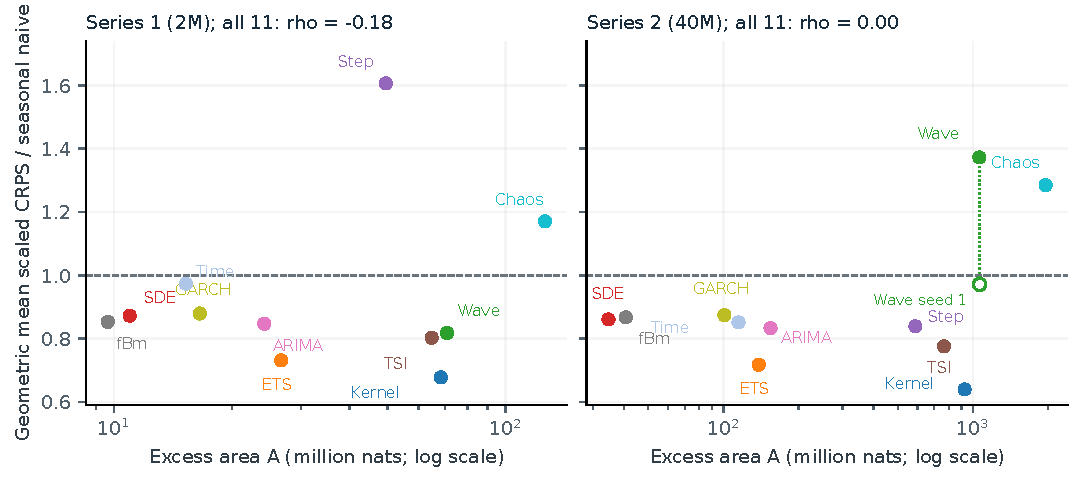
\includegraphics[width=\linewidth]{figures/transfer_results.pdf}
\caption{Area and transfer for every prior. The horizontal line is seasonal
naive. Waveform's extra initialization (open marker) changes aggregate CRPS
markedly despite an almost identical area. Horizontal axes are logarithmic.}
\label{fig:transfer}
\end{figure}

Selected subsets show stronger associations. Excluding Chaotic and StepFunction
gives $\rho=-0.73$ at 2M ($n=9$, interval $[-0.95,-0.14]$), but only $-0.28$
at 40M. Additionally excluding Waveform at 40M gives $-0.83$
($n=8$, $[-1.00,-0.24]$). The sensitivity analysis also explores fifteen
area variants. Such exclusions and metric choices are exploratory, selected
after seeing the results; they do not establish a universal ranking rule.

Waveform illustrates sensitivity to forecast tails. At 40M, a second
initialization gives almost identical areas (1061.2 versus 1063.6 million nats)
but CRPS ratios of 1.373 and 0.972. The median configuration ratios are much
closer (0.750 and 0.721). The worst seed-0 configuration,
\texttt{bitbrains\_rnd/5T/short}, has a CRPS ratio of about $2.67\times10^5$;
the same configuration gives 58.0 for seed 1. The saved summaries locate the
failure but do not expose its individual forecast samples. Replacing Waveform
seed 0 with seed 1 still leaves the full-set area correlation near zero
($\rho=0.009$).

The floor is a second sensitivity: ARIMA's 40M area falls from 154.5 to 15.4
million nats when using the raw endpoint. Full-set raw-floor correlations
are $-0.15$ and $+0.19$. An EMA endpoint therefore changes the measured amount
of structure substantially, without resolving the lack of a stable
full-set association.

\subsection{Short prefixes and a compression baseline}
The seven held-out checkpoints permit a first look at early prediction.
At each prefix, we recompute area using that checkpoint's own EMA floor,
and compare its ranking with final downstream CRPS
(Figure~\ref{fig:prefix}). We also compare checkpoint loss and the loss drop
from the mean loss in the initial 1\% of training steps. No future endpoint
loss enters a prefix estimate. Associations vary with budget and checkpoint;
this is an exploratory correlation analysis, without a predictor trained and
validated on unseen generator families.

\begin{figure}[htbp]
\centering
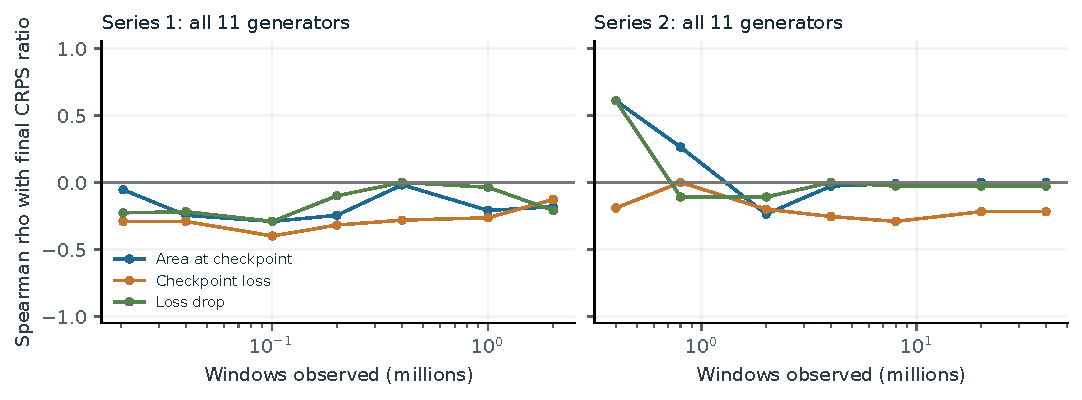
\includegraphics[width=\linewidth]{figures/prefix_results.pdf}
\caption{Prefix statistics versus final aggregate CRPS across all eleven priors.
Negative values favor larger predictor values. Checkpoints use their own floor;
the curves do not constitute an out-of-sample prediction test.}
\label{fig:prefix}
\end{figure}

The gzip baseline uses 5,000 series for each of ten priors (TimeSynth absent),
with raw float32 and range-normalized int16 rates. Int16-rate correlations with
CRPS are $-0.59$ at 2M and $-0.47$ at 40M; both intervals include zero.
Current uncertainty establishes no advantage for either proxy.

\section{Discussion and conclusion}
KernelSynth and ETS provide the strongest aggregate transfer in our comparison.
Excess prequential loss, however, does not consistently rank all eleven priors.
This limits its present use as a data-selection criterion: a large area measures
learning progress on the synthetic task, which need not capture the structure
needed by the downstream benchmark. Moreover, Eq.~\eqref{eq:area} makes area a
function of accumulated loss and the endpoint; it is not an independent source
of information once both are known.

The study uses one model configuration, mostly one initialization per prior,
and matched data budgets rather than measured equal-compute budgets. Subset
correlations and prefix analyses are exploratory. These constraints preclude
claims of architecture-independent epiplexity or a validated early transfer
predictor. Future studies should predeclare the floor and aggregation protocol,
repeat initializations, and validate prior selection on held-out generator
families. Oracle, noise-replacement, mixture, and model-size studies remain future
work. The current evidence supports useful prior choices under a fixed protocol,
but does not establish a general epiplexity-based ranking rule.

\clearpage
\bibliographystyle{plainnat}
\bibliography{references}

\clearpage
\appendix
\section{Evidence and reproducibility}
The archived training runs were conducted by Danila Chernousov
(\texttt{Chernousovdv}); this article analyzes the resulting shared experiment
artifacts. No training is rerun for the report analysis.

The analysis uses \texttt{experiments/episynth/series1\_2026-10-19/} and
\texttt{series2\_2026-10-19/} at commit \texttt{7d2b001}: run configurations,
training curves, held-out logs, and evaluation summaries. Scripts hash every
input. Training used RTX 4090/A100 hardware; KernelSynth's long series used a
GPU-generated float64 corpus. Its interrupted first checkpoint was recovered
from saved weights; exported steps are contiguous.

Batch means suffice for the linear signed area. Their six-significant-digit
export introduces a worst-case area rounding bound below 0.013 million nats.
All 22 primary estimates agree with the uploaded per-window analysis to its
displayed precision of 0.1 million nats. We did not download the release's large
per-window loss vectors or model weights. Consequently, we do not reconstruct
clipped per-window variants, held-out standard errors, or individual forecast
failures. Bootstrap intervals have no correction for the exploratory comparisons.

Saved seasonal-naive point metrics match the committed original leaderboard
on all 55 configurations, with maximum relative discrepancy below
$1.7\times10^{-7}$ across MASE, sMAPE, ND, MAE, and MSE. A fresh rerun of the
existing \texttt{tests/episynth} suite gives \ChecksPassed{} passed,
\ChecksSkipped{} skipped, and \ChecksFailed{} failed; the skips require external
GIFT-Eval data and the original Moirai checkpoint. These are report-time checks,
distinct from the archived training. An OU Bayesian-reference check is implemented
and covered by this rerun; no OU training/transfer run appears in the saved series.
The earlier Moirai-port agreement claim
($7\times10^{-4}$ nats/point) is reported in the author's implementation
commit~\cite{chernousovcode}, not independently remeasured here.

One unit convention deserves care: if context scaling uses $z=(y-\mu)/s$, then
$\mathrm{NLL}_{\rm raw}=\mathrm{NLL}_z+h\log s$.
Thus normalized NLL is raw NLL \emph{minus} $h\log s$; an existing training
docstring states the opposite sign. Our analysis retains raw-unit scores.

Rebuild statistics and tables with \texttt{analyze\_runs.py}, plots with
\texttt{make\_plots.py}, and the checked PDF with \texttt{build\_report.py}.
\texttt{reproduce.py} also reruns tests and records the environment.
Evidence is under \texttt{data/}; versions are pinned in \texttt{requirements.txt}.

\section{Implementation contracts for the four algorithms}
\label{sec:algorithms}
Code paths below are relative to \texttt{src/episynth/}; tests are under \texttt{tests/episynth/}.
\begin{enumerate}
\setlength{\itemsep}{1pt}
\setlength{\parskip}{0pt}
\item \textbf{Seeded task generation.} Given a prior, seed range and window
specification, generate series; use separate SplitMix64-derived streams to draw
context length, start and dequantization noise; patch and mask the result.
Output: \texttt{WindowBatch}. Code: \texttt{windows.make\_windows} and
\texttt{WindowStream}; tests: \texttt{test\_windows.py} and \texttt{test\_corpus.py}.
\item \textbf{Probabilistic training.} Evaluate and retain each window's NLL
before updating; optimize mean NLL per target point with AdamW, warmup and
gradient clipping; update EMA; checkpoint raw/EMA weights and score independent
held-out seeds. Output: weights and loss logs. Code: \texttt{training.Trainer};
tests: \texttt{test\_training.py}.
\item \textbf{Excess-loss estimation.} Sum pre-update window NLLs, subtract
$N$ times the selected held-out endpoint, retain the sign, and convert nats to
bits. With per-window held-out losses, report $N\,\mathrm{SE}(\widehat\ell_N)$;
batch-mean exports alone cannot supply that error. Code:
\texttt{analysis.run\_area}; report reconstruction: \texttt{analyze\_runs.py};
tests: \texttt{test\_analysis.py}.
\item \textbf{Transfer evaluation and ranking.} Generate forecasts on matched
GIFT-Eval windows; compute sample CRPS and point metrics; aggregate ratios to
seasonal naive by Eq.~\eqref{eq:quality}; correlate prior-level scores with area
using Spearman ranks and paired family bootstrap intervals. Output: configuration
scores, rankings and intervals. Code: \texttt{evaluation/} and \texttt{analysis.py};
tests: \texttt{test\_evaluation.py} and \texttt{test\_analysis.py}.
\end{enumerate}
\end{document}
